\documentclass[12pt,a4paper]{report}
\usepackage[utf8]{inputenc}
\usepackage{amsmath}
\usepackage{amsfonts}
\usepackage{amssymb}
\usepackage{graphicx}
\usepackage{lmodern}

\graphicspath{ {diagrams/} }

\newcommand*{\al}{\overline{A}}
\newcommand*{\bl}{\overline{B}}
\newcommand*{\cl}{\overline{C}}
\newcommand*{\dl}{\overline{D}}


\setlength{\parindent}{0cm}

\author{Kyle Swanson}
\title{Chapter 2 Exercises: Combinational Logic and Boolean Algebra }

\begin{document}
\maketitle

\begin{normalsize}

\textbf{2.2} Write a Boolean equation in sum-of-products canonical form for each of the truth tables in Figure 2.81. \\

To determine this, look where Y = 1. Then just put complemented or not A, B, C, or D AND'ED together (Ex: If B = 0, complement it.). That is, turn the inputs to 1. And OR the results. \\

(a) $ \al{}B = 1 $ , $ A\overline{B} = 1 $, $ AB = 1 $. Therefore \\ 
$ Y = \overline{A}B + A\overline{B} + AB $ \\

(b) $ Y = \overline{A}\overline{B}C + \overline{A}B\overline{C} + \overline{A}BC + A\overline{B}\overline{C} + AB\overline{C}$ \\

(c) $ Y = \overline{A}\overline{B}C + AB\overline{C} + ABC $ \\

(d) $ Y = \overline{A}\overline{B}\overline{C}\overline{D} + \overline{A}\overline{B}C\overline{D} + \overline{A}\overline{B}CD + \overline{A}BC\overline{D} + \overline{A}BCD + A\overline{B}\overline{C}\overline{D} + A\overline{B}C\overline{D} $ \\

(e) $ Y = \overline{A}\overline{B}CD + \overline{A}BC\overline{D} + \overline{A}BCD + A\overline{B}\overline{C}\overline{D} + A\overline{B}\overline{C}D + A\overline{B}C\overline{D} + A\overline{B}CD $ \\

\textbf{2.4} Write a Boolean equation in product-of-sums canonical form for the truth tables in 2.81. \\

To determine this, look where Y = 0. Then just put complemented or not A, B, C, or D OR'ED together (Ex: If B = 0, do not complement it.). That is, turn the inputs to 0. And AND the results. \\

(a) $ Y = (A + B) $ \\

(b) $ Y = (A + B + C) (\overline{A} + B + \overline{C}) (\overline{A} + \overline{B} + \overline{C}) $ \\

(c) $ Y = (A + B + C) (A + \overline{B} + C) (A + \overline{B} + \overline{C}) (\overline{A} + B + C) (\overline{A} + B + \overline{C}) $ \\

(d) $ Y = (A + B + C + \overline{D}) (A + \overline{B} + C + D) (A + \overline{B} + C + \overline{D}) (\overline{A} + B + C + \overline{D}) (\overline{A} + B + \overline{C} + \overline{D}) (\overline{A} + \overline{B} + C + D) (\overline{A} + \overline{B} + C + \overline{D}) (\overline{A} + \overline{B} + \overline{C} + D) (\overline{A} + \overline{B} + \overline{C} + \overline{D}) $ \\

(e) $ Y = (A + B + C + D) (A + B + C + \overline{D}) (A + B + \overline{C} + D) (A + \overline{B} + C + D) (A + \overline{B} + C + \overline{D}) (\overline{A} + \overline{B} + C + D) (\overline{A} + \overline{B} + C + \overline{D}) (\overline{A} + \overline{B} + \overline{C} + D) (\overline{A} + \overline{B} + \overline{C} + \overline{D}) $ \\

\textbf{2.6} Minimize each of the Boolean equations from Exercise 2.2. \\
(a) $ Y = \overline{A}B + A\overline{B} + AB $ \\
$ = \al{}B + A(\bl{}+B) $ T5'\\
$ = \al{}B + A $ \\
Finally, you can remove the $ \al{} $. Due to T1 or T2. See the examples below for justification.\\
$ = A + B $ \\
Examples on why $ \al{} $ can be eliminated. \\
A = 1, B = 1. $ 0\: and\: 1\: or\: 1 = 1 \Leftrightarrow 1\: or\: 1 = 1 $ \\
A = 0, B = 1. $ 1\: and\: 1\: or\: 0 = 1 \Leftrightarrow 1\: or\: 0 = 1 $ \\
A = 1, B = 0. $ 0\: and\: 0\: or\: 1 = 1 \Leftrightarrow 0\: or\: 1 = 1 $ \\
A = 0, B = 0. $ 1\: and\: 0\: or\: 0 = 0 \Leftrightarrow 0\: or\: 0 = 0 $ \\
See how they're the same? Since $ \al{} $ and B are AND'ed together, $ \al{} $ doesn't matter since it has A on the other side of an OR. \\

(b) $ Y = \overline{A}\overline{B}C + \overline{A}B\overline{C} + \overline{A}BC + A\overline{B}\overline{C} + AB\overline{C}$ \\
$ = \al{}(\bl{}C + B\cl{} + BC) + \cl{}(A\bl{} + AB) $ T8 \\
$ = \al{}(C(\bl{}+B) + B\cl{}) + A\cl{} $ T5, T3 \\
$ = \al{}(B\cl{} + C) + A\cl{} $ \\
$ = \al{}(B + C) + A\cl{} $ \\
$ = \al{}B + \al{}C + A\cl{} $ \\

(c) $ Y = \overline{A}\overline{B}C + AB\overline{C} + ABC $ \\
$ = \overline{AB}C + A(B(\cl{}+C)) $ \\ 
$ = \overline{AB}C + AB $ T5, T3 \\

(d) $ Y = \overline{A}\overline{B}\overline{C}\overline{D} + \overline{A}\overline{B}C\overline{D} + \overline{A}\overline{B}CD + \overline{A}BC\overline{D} + \overline{A}BCD + A\overline{B}\overline{C}\overline{D} + A\overline{B}C\overline{D} $ \\
$ = \overline{AB}(\overline{CD} + C\dl{} + CD) + \al{}BC(\dl{} + D) + A\overline{BD}(\cl{} + C)$ \\
$ = \overline{AB}(C + \dl{}) + \al{}BC + A\overline{BD}  $ \\
$ = \overline{AB}C + \overline{ABD} + \al{}BC + A\overline{BD} $ \\
$ = \overline{BD}(\al{} + A) + \al{}C(\bl{} + B) $ \\
$ = \al{}C + \overline{BD} $ \\

(e) $ Y = \overline{A}\overline{B}CD + \overline{A}BC\overline{D} + \overline{A}BCD + A\overline{B}\overline{C}\overline{D} + A\overline{B}\overline{C}D + A\overline{B}C\overline{D} + A\overline{B}CD $ \\
$ = $ \\


\textbf{2.8} Sketch a reasonably simple combinational circuit implementing each of the functions from Exercise 2.6. \\
(a) $ Y = A + B $ \\
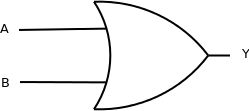
\includegraphics[scale=1]{2_8A} \\

(b) $ Y = \al{}B + \al{}C + A\cl{} $ \\
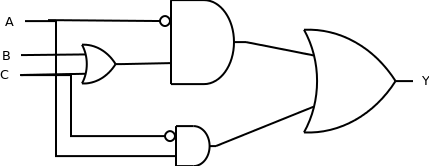
\includegraphics[scale=1]{2_8B} \\

(c) $ Y = \overline{AB}C + AB $ \\
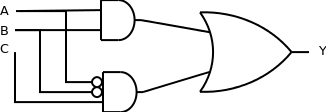
\includegraphics[scale=1]{2_8C} \\

(d) $ = \al{}C + \overline{BD} $ \\
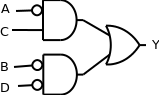
\includegraphics[scale=1]{2_8D} \\

(e) \\

\textbf{2.14} Simplify the following Boolean equations using Boolean theorems. Check for correctness using a truth table or K-map. \\

(a) $ Y = \overline{A}BC + \overline{A}B\overline{C} $ \\
$ = \al{}B(C + \cl{}) $ \\
$ = \al{}B $ \\ \\
\begin{tabular}{|c|c|c|c|c|}
A & B & C & $ \al{}BC+\al{}B\cl{} $ & $ \al{}B $ \\ 
\hline 
1 & 1 & 1 & 0 & 0 \\ 
\hline 
1 & 1 & 0 & 0 & 0 \\ 
\hline 
1 & 0 & 1 & 0 & 0 \\ 
\hline 
1 & 0 & 0 & 0 & 0 \\ 
\hline 
0 & 1 & 1 & 1 & 1 \\ 
\hline 
0 & 1 & 0 & 1 & 1 \\ 
\hline 
0 & 0 & 1 & 0 & 0 \\ 
\hline 
0 & 0 & 0 & 0 & 0 \\ 
\hline 
\end{tabular} \\

(b) $ Y = \overline{ABC} + A\overline{B} $ \\
$ = \bl{}(\overline{AC} + A) $ \\
$ = \bl{}(A + \cl{}) $ \\
$ = A\bl{} + \overline{BC} $ \\ \\
\begin{tabular}{|c|c|c|c|c|}
A & B & C & $ \overline{ABC} + A\overline{B} $ & $ A\bl{} + \overline{BC} $ \\ 
\hline 
1 & 1 & 1 & 0 & 0 \\ 
\hline 
1 & 1 & 0 & 0 & 0 \\ 
\hline 
1 & 0 & 1 & 1 & 1 \\ 
\hline 
1 & 0 & 0 & 1 & 1 \\ 
\hline 
0 & 1 & 1 & 0 & 0 \\ 
\hline 
0 & 1 & 0 & 0 & 0 \\ 
\hline 
0 & 0 & 1 & 0 & 0 \\ 
\hline 
0 & 0 & 0 & 1 & 1 \\ 
\hline 
\end{tabular} \\ \\


(c) $ Y = ABC\overline{D} + A\overline{BCD} + (\overline{A + B + C + D}) $ \\
$ = ABC\dl{} + A\overline{BCD} + \overline{ABCD} $ \\
$ = \dl{}(ABC + A\overline{BC} + \overline{ABC}) $ \\
$ = \dl{}(ABC + \overline{BC}(A + \al{})) $ \\
$ = \dl{}(ABC + \overline{BC}) $ \\
$ = ABC\dl{} + \overline{BCD} $ \\ \\
\begin{tabular}{|c|c|c|c|c|c|}
A & B & C & D & $ ABC\overline{D} + A\overline{BCD} + (\overline{A + B + C + D}) $ & $ ABC\dl{} + \overline{BCD} $ \\ 
\hline 
1 & 1 & 1 & 1 & 0 & 0 \\ 
\hline 
1 & 1 & 1 & 0 & 1 & 1 \\ 
\hline 
1 & 1 & 0 & 1 & 0 & 0 \\ 
\hline 
1 & 1 & 0 & 0 & 0 & 0 \\ 
\hline 
1 & 0 & 1 & 1 & 0 & 0 \\ 
\hline 
1 & 0 & 1 & 0 & 0 & 0 \\ 
\hline 
1 & 0 & 0 & 1 & 0 & 0 \\ 
\hline 
1 & 0 & 0 & 0 & 1 & 1 \\ 
\hline 
0 & 1 & 1 & 1 & 0 & 0 \\ 
\hline 
0 & 1 & 1 & 0 & 0 & 0 \\ 
\hline 
0 & 1 & 0 & 1 & 0 & 0 \\ 
\hline 
0 & 1 & 0 & 0 & 0 & 0 \\ 
\hline 
0 & 0 & 1 & 1 & 0 & 0 \\ 
\hline 
0 & 0 & 1 & 0 & 0 & 0 \\ 
\hline 
0 & 0 & 0 & 1 & 0 & 0 \\ 
\hline 
0 & 0 & 0 & 0 & 1 & 1 \\ 
\hline 
\end{tabular} \\ \\


\textbf{2.16} Sketch a reasonably simple combinational circuit implementing each of the functions from Exercise 2.14.\\
(a) $ = \al{}B $ \\
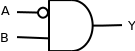
\includegraphics[scale=1]{2_16A} \\

(b) $ = A\bl{} + \overline{BC} $ \\
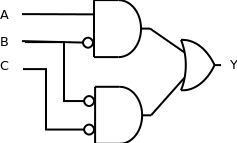
\includegraphics[scale=1]{2_16B} \\

(c) $ ABC\dl{} + \overline{BCD} $ \\
TODO! Add the picture \\

\textbf{2.22} Prove that the following theorems are true using perfect induction. You need not prove their duals.\\

For these, build a truth table. Show every option. And so long as the theorem matches with what it claims, it is proved. \\

(a) The idempotency theorem (T3), $ B \bullet B = B $ \\
See how '$ B $' matches '$ B \bullet B $'? \\ \\
\begin{tabular}{|c|c|}
$ B $ & $ B \bullet B $ \\ 
\hline 
0 & 0 \\ 
\hline 
1 & 1 \\ 
\hline 
\end{tabular} \\ \\

(b) The distributivity theorem (T8), $ (B \bullet C) + (B \bullet D) = B \bullet (C + D) $ \\ \\
\begin{tabular}{|c|c|c|c|c|}
B & C & D & $ (B \bullet C) + (B \bullet D) $ & $ B \bullet (C + D) $ \\ 
\hline 
1 & 1 & 1 & 1 & 1 \\ 
\hline 
1 & 1 & 0 & 1 & 1 \\ 
\hline 
1 & 0 & 1 & 1 & 1 \\ 
\hline 
1 & 0 & 0 & 0 & 0 \\ 
\hline 
0 & 1 & 1 & 0 & 0 \\ 
\hline 
0 & 1 & 0 & 0 & 0 \\ 
\hline 
0 & 0 & 1 & 0 & 0 \\ 
\hline 
0 & 0 & 0 & 0 & 0 \\ 
\hline 
\end{tabular} \\ \\

(c) The combining theorem (T10), $ (B \bullet C) + (B \bullet \cl{}) = B $ \\ \\
\begin{tabular}{|c|c|c|c|}
B & C & $ (B \bullet C) + (B \bullet \cl{}) $ & B \\
\hline 
1 & 1 & 1 & 1 \\ 
\hline 
1 & 0 & 1 & 1 \\ 
\hline 
0 & 1 & 0 & 0 \\ 
\hline 
0 & 0 & 0 & 0 \\ 
\hline 
\end{tabular} \\ \\

\end{normalsize}

\end{document}























